\documentclass[11pt]{article}
\usepackage[a4paper,margin=24mm]{geometry}
\usepackage{amsmath,amssymb,amsthm,booktabs,graphicx,xcolor,hyperref}
\hypersetup{colorlinks=true,linkcolor=blue!50!black,urlcolor=blue!50!black,citecolor=blue!50!black,pdftitle={Boundary augmentation and symmetric interpolation for no-three-in-line sets}}
\newtheorem{theorem}{Theorem}[section]\newtheorem{lemma}[theorem]{Lemma}\newtheorem{proposition}[theorem]{Proposition}\newtheorem{corollary}[theorem]{Corollary}
\newcommand{\F}{\mathbb F_p}\newcommand{\Z}{\mathbb Z}\newcommand{\B}{\mathcal B}\newcommand{\D}{\mathcal D}\newcommand{\A}{\mathcal A}\newcommand{\ch}{\chi}\newcommand{\eps}{\varepsilon}
\title{Boundary augmentation and symmetric interpolation for no-three-in-line sets}
\author{Unsigned working draft for independent review}
\date{19 November 2026}
\begin{document}\maketitle
\begin{abstract}\noindent
For each prime $p\equiv1\pmod{24}$ we construct a half-turn invariant set of $6p+2$ points with no three collinear on the ordinary square grid of side $4p+1$. The construction adjoins eight boundary points to a previously known four-period conic ring. The excess over $3n/2$ is $1/2$. A positive proportion of nonsquare conic levels suffice asymptotically, with an explicit lower bound. For any prime $p>3$ and $3p\le n\le4p$ we also construct a half-turn invariant set of at least $2n-2p-16$ points. A change of level eliminates the loss from exceptional residue classes when $4p-n\ge32\sqrt p$. The bounds do not increase the leading coefficient $3/2$ in the unrestricted problem.
\end{abstract}

\section{Results and relationship to prior work}
A \emph{cap} is a finite subset of $\Z^2$ containing no three distinct points on an ordinary line. Write $F(n)$ for the maximum size of a cap on $[0,n-1]^2\cap\Z^2$, and $F_{\rm ht}(n)$ for the maximum when the cap is invariant under $(x,y)\mapsto(n-1-x,n-1-y)$. Hall, Jackson, Sudbery and Wild \cite{hjsw} obtained $3(p-1)$ points at $n=2p$ and hence $F(n)\ge(3/2-o(1))n$. For a recent treatment see \cite[Theorems 1.2 and 2.8]{kns}. This leading coefficient is not a contribution of this work.

\begin{theorem}[Boundary augmentation]\label{thm:boundary}
For every prime $p\equiv1\pmod{24}$, $F_{\rm ht}(4p+1)\ge6p+2$. The $6(p-1)$ original points are all retained. For $p\equiv1\pmod{840}$ every nonsquare level works, with no finite checks. In general the fraction of nonsquare levels that work has lower limit at least $(2/5)^4(6/7)^4$ along primes $1\pmod{24}$.
\end{theorem}
For the full progression the proof of existence is analytic for $p>50625$; a small exact certificate handles the rest. The fraction statement is analytic. The $3n/2+1/2$ lower bound occurs on an infinite sequence, not on all sides.

\begin{theorem}[Rectangular interpolation]\label{thm:rect}
Let $p>3$ be prime and $3p\le n\le4p$. Define
\[
 B(n,p)=2n-2p-\begin{cases}4,&n\text{ odd},\\6,&n\text{ even}.\end{cases}
\]
A cap invariant under the board's half-turn has size at least $B(n,p)-\delta$, where $\delta=0$ if $p\equiv1\pmod{12}$, $\delta=8$ if $p\equiv5\pmod{12}$, and $\delta=10$ if $p\equiv3\pmod4$. If $4p-n\ge32\sqrt p$, a cap of size $B(n,p)$ can be constructed in every prime class.
\end{theorem}
The last statement concerns a construction count, not the optimum. Choosing the first prime $p\ge n/4$ for large $n$ yields $F_{\rm ht}(n)\ge(3/2-o(1))n$. Alternatively, if $p<q$ are consecutive large primes and $4p\le n\le4q$, centring the $4p$ or $4p-1$ cap according to parity gives $6p-16$, and using $q$ gives $2n-2q-16$ (since $n\ge3q$ eventually). Taking the larger gives the uniform error bound
\[
 F_{\rm ht}(n)\ge\tfrac32n-\tfrac32(q-p)-16.
\]
Indeed $\min\{3(n-4p)/2,2q-n/2\}\le3(q-p)/2$. In particular the published prime-gap estimate of Baker, Harman and Pintz \cite{bhp} yields $F_{\rm ht}(n)\ge3n/2-O(n^{0.525})$ for all large $n$. This is a prime-gap corollary, not a larger density coefficient. The sets for different sides need not be nested. The leading asymptotic alone is not the point: the exact four-period masks at primes $1\pmod{12}$, with the appropriate parity of the containing board and ordinary prime rounding, already suffice for that.

\paragraph{Attribution and scope.} The two six-site outer masks, the physical parity rule, the signed multiplicative-coset colouring and local interface trims come from the four-period construction of cedar\_conics and lattice\_lift\_research \cite{ring}; empirical masks are credited there to \cite{map}. We use those facts below, with proofs for the forms needed. Our additions are protected off-carrier boundary placements, a count of sufficient levels, rectangular repairs and the relocation of exceptional classes. Kudriashov \cite{window} treats extremal subsets of the carrier in a $2p$ window. Finite insertions into other starting sets were reported in \cite{insertions}. The computer-assisted upper bound of \cite{ladder} for a single translated carrier on $3p\le n<4p$ limits the leading coefficient of the rectangular approach; it does not preclude these lower bounds or the eight off-carrier points. We do not assert priority for all possible constructions with comparable counts.

\section{The ring and its boundary}
Let $p\equiv1\pmod{24}$, let $k$ be a quadratic nonresidue, and write $e(u)=(1-\ch(u))/2$ for $u\ne0$, where $\ch$ denotes the quadratic character. In $[0,4p]^2$ take $O$ to consist of the integer sites satisfying
\[
 xy\equiv k\pmod p,\qquad x+y\equiv e(x)\pmod2,\qquad (\lfloor x/p\rfloor,\lfloor y/p\rfloor)\notin\{1,2\}^2.
\]
The character is evaluated modulo $p$ before the parity comparison. Points with the same two residues form a \emph{fibre}. With $u,v\in[1,p-1]$ representing $u,k/u$, its lifts are $(u+ip,v+jp)$ and its \emph{sheet indices} $(i,j)$ are one checkerboard half of the twelve outer cells in a $4\times4$ square:
\begin{align*}
 M_0&=\{00,02,13,20,31,33\}, & M_1&=\{01,03,10,23,30,32\}.
\end{align*}
Here $ij$ denotes $(i,j)$, and the subscript is $i+j\bmod2$. Each list is a cap; its only nonaxis primitive pair directions, up to a common sign, are
\[
 \D=\{(1,\pm1),(1,\pm3),(3,\pm1)\}.                 \tag{1}
\]
These statements follow by subtracting the six entries pairwise.

A primitive integer line reduces to a line over $\F$ and meets $xy=k$ in at most two residues. Any triple would have a same-fibre pair. An axis cannot then meet another fibre. For a pair of primitive direction $(a,b)\in\D$, the other residue on the line has first coordinate
\[
 u'=-ak/(bu),                                             \tag{2}
\]
by the product of the two roots after substitution. Since $-1$ and $3$ are squares here, $e(u')=1-e(u)$. Physical parity is constant on this odd--odd line, so it cannot supply a triple. Thus $O$ is a cap of size $6(p-1)$. The reflection $(x,y)\mapsto(4p-x,4p-y)$ preserves it since $\ch(-1)=1$.

\paragraph{Boundary rays.} On each edge choose two of its three open-side sites in $p\{0,1,2,3,4\}^2$. The eight chosen sites are a cap by convexity and the edge count. The orbit of $(0,p)$ under all square symmetries is a half-turn invariant choice. Any nonaxis line through two of these sites has primitive height $H=\max(|a|,|b|)\le4$. From a coarse site $q$ every lattice site on the line is $q+t(a,b)$ and the carrier condition is
\[
                         abt^2\equiv k\pmod p.             \tag{3}
\]
For $H\le4$, all signed products $ab\ne0$ are squares because $-1,2,3$ are squares, so no such line meets the carrier. A coarse axis does not meet it either.

A nonaxis line through one open-side site has only one inward ray, with positive $t\le4p/H$. For $H\ge8$ this interval has length at most $p/2$, so at most one of the two opposite roots of (3) occurs. If $p\mid ab$ there is none. For $5\le H\le7$ and $a+b$ odd, the two possible parameters $r,p-r$ have opposite parity. Their $x$-residues are negatives with equal character, so at most one site belongs to $O$. In the odd--odd case it suffices that the least positive root up to sign obey
\[
                      Hr<(H-4)p.                          \tag{4}
\]
Indeed the other root then exceeds the ray length. For $p\equiv1\pmod{840}$ the primes $2,3,5,7$ and $-1$ are squares, so (3) has no roots for any $H\le7$. This proves the elementary subprogression in Theorem~\ref{thm:boundary}.

\paragraph{Existence of a level.} The signed odd--odd products potentially requiring (4) are $\pm5,\pm15$ at height five and $\pm7,\pm21,\pm35$ at height seven; discard squares. Fix a nonsquare $\nu$ and roots $s_d^2=\nu/d$ for the retained products $d$. Use $b_d=5$ at height five and $b_d=3$ at height seven, and $J=\prod b_d$. Divide each coordinate of a unit cube into $b_d$ equal parts. Two of the $J+1$ vectors $(\{js_d/p\})_d$, $0\le j\le J$, are in one box; the nonzero index difference $z\le J$ satisfies $\|zs_d/p\|<1/b_d$ in every coordinate. If $p>J$, then $k=\nu z^2$ works since $1/3<3/7$. For the empty list take $k=\nu$. By the signs of $\ch(5),\ch(7)$, $J$ is one of $1,729,5625,50625$.

For the 194 remaining primes $p\equiv1\pmod{24}$, $p\le J(p)$, the ancillary table gives a nonsquare $k$ in each case. In 191 cases (4) is checked directly for each retained product. At $(p,k)=(73,28),(97,17),(193,20)$ the exact checker constructs $O$, tests all normalized directions from each of the twelve open-side sites to $O$ for duplicates, and checks that every two-anchor line misses $O$. The checker independently sieves the prime range and verifies completeness of the table. This proves the finite assertion. All $3^4$ labelled edge choices work, of which nine are invariant under the half-turn.

\begin{figure}[ht]\centering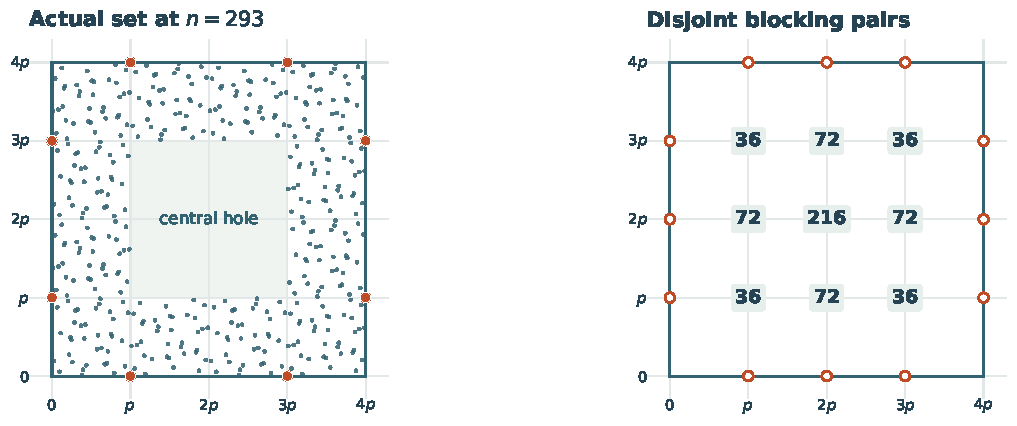
\includegraphics[width=.84\linewidth]{ring.pdf}\caption{Left: the $432+8$ construction at $p=73$. Right: numbers of disjoint pairs of old points reflected into one another about the nine interior coarse sites. The twelve open-side candidates are shown as circles.}\label{fig:ring}\end{figure}

\paragraph{A limitation on coarse insertions.} A pair of old points symmetric about $p(i,j)$ blocks that insertion, and all such pairs about one site are disjoint. In sheet coordinates reflection sends $(a,b)$ to $(2i-1-a,2j-1-b)$ in the negative fibre. The negative fibre uses the same mask, and exactly half the fibres use each mask: $u\leftrightarrow k/u$ preserves the least-residue sum and flips the character. Counting intersections of the displayed $M_t$ with their reflections gives the following array of pair counts at the nine interior coarse points:
\[
 \frac{p-1}{2}\begin{pmatrix}1&2&1\\2&6&2\\1&2&1\end{pmatrix}.
\]
Thus fewer than $(p-1)/2$ deletions cannot open an interior coarse site. The four edges allow at most eight boundary sites. This proves optimality of eight for this particular grid of candidates, not for all lattice sites.

\subsection{Abundance of sufficient levels}
Put $a=2/5$ and $b=6/7$. Along any one of the four quadratic-character patterns below, the proportion of nonsquare levels satisfying (4) for \emph{all} retained products converges to the indicated number. These are sufficient proportions, not the exact proportions of all legal levels.
\begin{center}\begin{tabular}{cccl}\toprule
$\ch(5)$ & $\ch(7)$ & limiting proportion & positive-product root multipliers, up to rational factors\\\midrule
$+$ & $+$ & $1$ & no constraints\\
$-$ & $+$ & $a^4b^2$ & $1,\sqrt3,\sqrt7$\\
$+$ & $-$ & $b^6$ & $1,\sqrt3,\sqrt5$\\
$-$ & $-$ & $a^4b^4$ & $1,\sqrt3,\sqrt{35},\sqrt{105}$\\\bottomrule\end{tabular}\end{center}
To see this choose $\nu=5$ if 5 is a nonsquare, otherwise $\nu=7$ if 7 is a nonsquare. Represent each $s_d$ by the reduction of $\gamma_d=\sqrt{\nu/d}$ in the relevant multiquadratic field. For negative $d$ the multiplier acquires $\sqrt{-1}$. The entries in a row, including these extra imaginary multiples, are linearly independent over $\mathbb Q$: they are distinct basis radicals of $\mathbb Q(\sqrt{-1},\sqrt3,\sqrt D)$ for $D=7,5,35$ respectively, up to nonzero rational factors. The needed radicals exist modulo each prime of the indicated pattern; signs may be chosen consistently.

For a fixed nonzero integer vector $h$, $\sum h_d\gamma_d\ne0$. Clearing denominators and taking its algebraic norm gives a fixed nonzero integer. Apart from primes dividing it or the denominator, $\sum h_d s_d\ne0\pmod p$. The average over $z\in\F$ of $\exp(2\pi i z\sum h_ds_d/p)$ is then zero. By Weyl's criterion the vectors $(\{z s_d/p\})_d$ become uniformly distributed in the unit torus along the pattern. Condition (4) cuts out intervals of measure $a$ or $b$ in the respective coordinates. Omitting $z=0$ changes nothing in the limit and each nonsquare $k=\nu z^2$ is counted twice, with the same test. This gives the table and the lower limit in Theorem~\ref{thm:boundary}. For example, at $p=200017$ the sufficient test accepts $1378$ of $100008$ nonsquare levels, compared with the limiting fraction $20736/1500625$ for that pattern.

\section{Rectangular fibre repairs}
Let $2\alpha=n-1\pmod p$. Use the translated carrier $(x-\alpha)(y-\alpha)=c\pmod p$. Fibre $u$ consists of $x=x_0+pi$, $y=y_0+pj$, with $x_0,y_0$ the least residues of $\alpha+u,\alpha+c/u$. The sheets form a $w\times h$ rectangle, $w,h\in\{3,4\}$. The half-turn exchanges $u,-u$; we select a mask on one fibre and reflect its points to the other. A signed vertex means $[u]=\{u,-u\}$ in $G=\F^*/\{1,-1\}$.

For a colour $T([u])\in\{0,1\}$, impose physical parity $T([u])$ on the selected points. The sheet parity is $T([u])-x_0-y_0\pmod2$. Only axes and the directions (1) are allowed within a mask. Formula (2) now uses $c$ in place of $k$. If its other fibre has a different colour, there is no triple. If $u'=u$ the line is tangent and only the original fibre matters. For any other same-colour partner, it suffices to forbid the corresponding repeated direction in the masks at both ends. This sufficient rule, unlike the wholesale removal of exceptional fibres, preserves part of each mask.

\begin{lemma}[Small templates]\label{lem:templates}
Each sheet colour admits a cap of $w+h-2$ with the allowed directions. If either $A=\{(3,\pm1)\}$ or $C=\{(1,\pm3)\}$ is additionally forbidden, at most one point of this size is lost, and if both are forbidden at most two are lost. In a square of side $w$, forbidding $(1,1)$ and either one of $A,C$ permits at least $w$ sites in sheet parity $0$ for $w=3$, or $1$ for $w=4$.
\end{lemma}
\begin{proof} Here are witnesses. In each pair the first list has even, the second odd sheet parity. For $3\times3$ use $00,02,20,22$ and $01,10,12,21$; neither high family occurs. For $3\times4$ use $00,02,13,20,22$ and $01,03,10,21,23$; neither uses $A$. To forbid both high families use $00,02,20,22$ and $01,03,21,23$. Transpose for $4\times3$. For $4\times4$ use $M_0,M_1$; when $A$ or $C$ is banned use the corresponding five-site $3\times4$ template or its transpose; when both are banned use its four-site template. For the last assertion with $A$ banned use $00,02,20$ in the small square and $03,10,23,30$ in the large one; transpose when $C$ is banned. Pairwise differences and ordinary determinants verify the lists.\end{proof}

\paragraph{The nominal count.} Omitting the unique coordinate residue $\alpha$ removes $\mu$ columns and $\mu$ rows. Here $\mu=3$ for odd $n$ and $4$ for even $n$: half-turn pairs columns in that residue, with a fixed column exactly when $n$ is odd. Hence summing $w+h-2$ over the $p-1$ fibres gives exactly $2(n-\mu)-2(p-1)=B(n,p)$.

For $p\equiv1\pmod{12}$ any nonsquare $c$ and $T([u])=e(u)$ suffice by (2), so there is no loss. In the other two cases choose a parameter $t\ne0$ (one may first take $t=1$). Put $K=\langle[3]\rangle$ in $G$, $L=|K|$. For $p\equiv3\pmod4$ the order of $G$ is odd. For $p\equiv5\pmod{12}$ the order of $K$ is even and the index $[G:K]$ is odd, since $-1$ is a square and $3$ is a nonsquare in the cyclic group of residues. In both cases choose $[c]$ in $[t]^2K$. On $G/K$ the involution $g\mapsto[c]/g$ has the unique fixed coset $[t]K$, since squaring is a bijection in this odd-order quotient. Other cosets can be paired and given opposite colours. All partners in (2) go to the opposite coset. It remains to colour just $[t]K$, indexed by $[t3^i]$, $i\in\Z/L\Z$.

\paragraph{Even cycle, $p\equiv5\pmod{12}$.} Choose $c=t^2/3$ and write $L=2h$. The three maps on indices are $i\mapsto-1-i+s$, $s=0,1,-1$; the two nonzero shifts belong to the two high direction families. Colour $0,\ldots,h-1$ zero and $h,\ldots,2h-1$ one. The unshifted map always changes colour. For $s=1$ the only same-colour incidences are the fixed vertices $0,h$; for $s=-1$ they are $h-1,2h-1$. At a fixed signed vertex the actual other residue is either $u$ (tangent) or $-u$. Suppress the indicated high family at this vertex. Count one lost site per actual fibre per incidence by Lemma~\ref{lem:templates}; if two incidences coincide, its two-family bound applies. Thus at most eight sites are lost.

\paragraph{Odd cycle, $p\equiv3\pmod4$.} Choose $c=t^2$, write $L=2h+1$. Here $L\ge3$ since $p>3$. The maps are $i\mapsto-i+s$ for $s=0,1,-1$. Give colour zero to $1,\ldots,h$ and one to $-h,\ldots,-1$. The unshifted map changes colour except at zero. Of the shifted maps, one has a fixed signed vertex at $h$, and the other at $-h$. In addition, precisely one of the edges $\{0,1\},\{0,-1\}$ is monochromatic, according to the choice of colour at zero. There are no other defects: for $1\le i\le h$ inspect $-i,-i+1,-i-1$ and use the reflected list on the other half.

At zero, $u=\pm t$ has $c/u=u$. The only dangerous unit-slope direction there is $(1,1)$, since the negative slope is tangent. This fibre is square with $x_0=y_0$. Choose its colour to give the preferred sheet parity in Lemma~\ref{lem:templates}. Banning the positive diagonal and the high family of the monochromatic edge costs at most $2$ sites per actual fibre at zero. Ban the same high family at the other endpoint, and the appropriate single high family at each shifted fixed vertex. These three incidences cost at most $1$ each per actual fibre, also when the noncentral endpoint coincides with a shifted fixed vertex ($L=3$). The total loss is at most $2(2+1+1+1)=10$. This proves the uniform part of Theorem~\ref{thm:rect}.

\subsection{Moving every defect into a short rectangle}
Write $d=4p-n$. The following observation also keeps track of the parity of the side. If $2u\equiv z\pmod p$, $|z|<d$, and $z\equiv n-1\pmod2$, the column residue $\alpha+u$ has width three. Indeed $2x-(n-1)$ on this residue is $z\pmod{2p}$; only $z,z\pm2p$ belong to $[-(n-1),n-1]$. The same applies to heights and to $-u$.

\begin{lemma}\label{lem:lattice}
Let $D\in\{-1,3,-3\}$ and $r^2\equiv D\pmod p$. For either prescribed common parity there is a nonzero vector $(z,w)$ of that parity in both coordinates, with $w\equiv rz\pmod p$ and $\max(|z|,|w|)<3\sqrt p$.
\end{lemma}
\begin{proof} The lattice of this congruence has determinant $p$. A shortest Euclidean vector $v$ satisfies $\sqrt{p/3}\le|v|\le\sqrt{2p}$. Indeed $w^2-Dz^2$ is a nonzero multiple of $p$ for every nonzero lattice vector, and the upper bound follows from Minkowski's theorem on a square of radius $\sqrt p+\epsilon$. For even parity take $2v$. Otherwise extend the primitive lattice vector $v$ to a basis $v,w_0$; reduce the projection of $w_0$ onto $v$ to length at most $|v|/2$. Then $|w_0|^2\le p^2/|v|^2+|v|^2/4\le 7p/2$. The determinant is odd, so one of $v,w_0,v+w_0$ has both coordinates odd. In the last case use the shorter of $v\pm w_0$, of norm at most $\sqrt{|v|^2+|w_0|^2}<3\sqrt p$.\end{proof}

For $p\equiv5\pmod{12}$ take $r^2=-1$ in $\F$. The four exceptional signed vertices, and their reciprocals under $c/u$, are represented up to sign by $t,t/3,rt,rt/3$: indeed $[3]^h$ is the nonidentity element of order two in $G$ and is represented by $\pm r$. For $p\equiv3\pmod4$ take $r=3^{h+1}$. Then $r^2=\pm3$ since $3^L=\pm1$. The indices $0,1,-1,h,-h$ and their reciprocals are represented up to sign by
\[
                         t,\quad 3t,\quad t/3,\quad rt,\quad rt/3.
\]
This includes both neighbours of zero, whether or not the edge to them was monochromatic.

In either case choose the vector of Lemma~\ref{lem:lattice} in parity $n-1$, and set $2s=z$, $t=3s$ in $\F$. Under $d\ge32\sqrt p$, $p\ge1024$ and neither coordinate of this nonzero vector can vanish modulo $p$. Twice each required signed coordinate has a representative among the signed odd multiples, of magnitude at most nine times $\max(|z|,|w|)$, of $z$ or $w$. Each representative has parity $n-1$ and absolute value $<d$. Every exceptional fibre just listed is therefore $3\times3$.

Both ordinary $3\times3$ templates have only axis and unit-slope pairs, so all high-family defects now cost nothing. In the odd-cycle case replace the mask of one fibre at zero by $\{01,02,11,12\}$ and reflect it to the mate. This unit square uses \emph{both} parities. The positive-diagonal offsets $j-i$ are $1,2,0,1$; the reflected offsets about the physical diagonal are their negatives. Thus a physical diagonal through the combined pair has at most two points. The negative diagonal is tangent. No pair in this unit square has a high direction; conversely the only other fibres that could send a high-direction pair into it have signed indices $[3t]$ or $[t/3]$. These are $3\times3$ and send no such pair. Axis lines cannot cross fibres. Hence the mixed-parity exception introduces no triple and has the full four sites per fibre. This proves the last part of Theorem~\ref{thm:rect}.

\section{Finite gains and verification}
For each of four fixed choices from Theorem~\ref{thm:boundary}, mark every lattice site on a line determined by two seed points. The unmarked sites are all individually legal insertions (the seed itself is excluded). We selected a mutually compatible half-turn invariant subfamily; the coordinates in the supplement certify the following lower bounds.
\begin{center}\begin{tabular}{rrrrrr}\toprule
$p$&$k$&side $n$&seed&individually legal&augmented cap\\\midrule
73&28&293&440&8&446\\97&17&389&584&12&594\\1009&11&4037&6056&184&6176\\2521&11&10085&15128&344&15364\\\bottomrule\end{tabular}\end{center}
A stand-alone checker, with no modular assumptions, compares normalized unoriented directions from every point to every other point. The four augmented sets passed $274724644$ such direction checks in total. A separate run on 712 rectangular examples passed $146705252$ direction checks. The $\sqrt p$ argument is not inferred from tests: examples on either side parity with $p=5003,5009$ were also checked using all primitive directions of height at most three, sufficient for a triple on the verified single conic in a window of side at most $4p$. These are not assertions of finite records or of a growing surplus over $3n/2$.

The four final sizes are exact if the specified seed is frozen and only half-turn invariant additions are allowed. For reproducibility there is a solver-independent upper check. The complete unmarked lists split into $4,6,92,172$ opposite pairs. Join two pairs if their union with at most one seed point contains a triple; there are $2,1,82,114$ such graph edges. From every remaining physical line on three new points, forbid its three distinct orbits if not already excluded by an edge; this adds $0,0,4,7$ distinct ternary constraints. An independent-set recursion branches on an unresolved ternary by deleting one of its three vertices, and when only graph edges remain, splits components and branches on inclusion or exclusion of a vertex. The exact packing numbers in orbits are $3,5,60,118$, attained by the supplied coordinates. Without freezing the seed, neither this upper bound nor the candidate list applies.

\appendix\section{A prime-rounding comparison on a positive density of sides}
For $n\ge6$ put $H(n)=3(P(n/2)-1)$, with $P(x)$ the largest prime at most $x$. It is sometimes useful to quantify the benefit of working on the $n/4$ scale instead of just this $n/2$ benchmark. The following observation already works, with adjusted constants, using the old four-period ring without the eight insertions; it is not a density-coefficient improvement.

\begin{proposition}There is an absolute $c>0$ such that in every sufficiently large dyadic interval $[Y,2Y]$ a positive absolute fraction of sides $n$ admit an embedded cap from Theorem~\ref{thm:boundary} of size at least $H(n)+c\log n$. They include disjoint intervals of $\gg\log Y$ consecutive such sides using a single embedded cap on each interval.\end{proposition}
\begin{proof} We give the uniform sieve input for clarity. For $a=1,2$ and $0<|j|\le\log X$, the count of integers $X<m\le3X/2$ with both $m,am+j$ prime is
\[
 \ll \frac{X}{(\log X)^2}\left(\frac{2|j|}{\varphi(2|j|)}\right)^2.
\]
Indeed sieve the product $m(am+j)$ by primes $\ell\nmid 2j$, $\ell\le z=X^{1/10}$. There are two roots at each sieving prime and squarefree remainders of size at most $2^{\omega(d)}$. Selberg's upper-bound sieve \cite[Theorem 1.1]{oh} gives a main term $O(X/G)$ with $G=\sum_{d\le z}\mu^2(d)\prod_{\ell\mid d}2/(\ell-2)$, restricted to allowed primes. The error is $O(z^{2+o(1)})$: the elementary Selberg weights at $d\le z$ have magnitude at most $\prod_{\ell\mid d}\ell/(\ell-2)=z^{o(1)}$, by their formula, and $2^{\omega(d)}=z^{o(1)}$ for $d\le z^2$. To bound $G$ from below restrict the Euler product to primes $\ell\le z^{\eta}$ for small fixed $\eta>0$. Under its normalized product weights a prime is selected with probability $2/\ell$. Thus $\mathbb E\log d\le 2\sum_{\ell\le z^{\eta}}(\log\ell)/\ell<\tfrac12\log z$ for large $X$. At least half the mass has $d\le z$. By Mertens' product estimate the mass is $\gg(\log X)^2(\varphi(2|j|)/(2|j|))^2$; the discrepancy in replacing $1-2/\ell$ by $(1-1/\ell)^2$ is bounded by a convergent positive product for $\ell>2$. This gives the stated bound. Also $\sum_{1\le j\le L}(2j/\varphi(2j))^2\ll L$, by expanding the product over primes dividing $j$ and summing multiples of each squarefree divisor (the resulting Euler product has terms $1+O(1/\ell^2)$).

Now set $X=Y/4$, $L=\lfloor\eta'\log X\rfloor$ with a sufficiently small absolute $\eta'>0$. The prime number theorem in progressions gives $\gg X/\log X$ primes $p\equiv1\pmod{24}$ in $(X,3X/2]$. Discard a $p$ if $2p+j$ is prime for $|j|\le L$, or if $p+j$ is prime for $1\le j\le L$; $2p$ itself is composite. Dropping the progression restriction in counting the discarded primes and summing the sieve bound gives $O(LX/(\log X)^2)$. Still $\gg X/\log X$ primes remain. They are spaced more than $L$ apart. For each of them $I_p=[4p+1,4p+2L]$ lies in $[Y,2Y]$; these intervals are disjoint. Throughout $I_p$, $P(n/2)\le2p-L-1$, so our $6p+2$ points exceed $H(n)$ by at least $3L+8$. Their intervals have total length $\gg Y$.\end{proof}

\paragraph{Why the unqualified benchmark gain is not new.} If only $F(n)$ matters and not the family furnishing the witness, even the preceding logarithmic advantage on a positive fraction follows by cropping the classical construction. For consecutive odd primes $q<r$, put $g=r-q$. Crop a classical cap on $2r$ to side $2r-d$, $1\le d\le g/2$. At most $4d$ points are deleted, since every row and every column has at most two. Thus $F(2r-d)\ge3(r-1)-4d\ge H(2r-d)+g$. Over consecutive gaps inside $[Y/2,Y]$ their total length is $(1/2-o(1))Y$ by the prime number theorem. Gaps smaller than $c_0\log Y$ contribute at most $O(c_0Y)$ since there are $O(Y/\log Y)$ primes. The remaining gaps supply the claimed positive fraction for sufficiently small fixed $c_0$. One may crop once at the smallest side of each interval and embed that one set throughout. What the proposition adds is a comparison for a specified, different family, not an unrestricted novelty claim.

\paragraph{Use of computational tools.} Arena.ai's Agent Mode was used substantially in proposing the constructions and proofs, writing the search and verification programs, performing computations and drafting the text. This unsigned research draft makes no representation of completed human review. The auxiliary search used OR-Tools CP-SAT; neither the geometric witness checks nor the upper-bound recursion use a solver. Machine cross-checks are not peer review.

\begin{thebibliography}{99}\small
\bibitem{hjsw} R. R. Hall, T. H. Jackson, A. Sudbery and K. Wild, Some advances in the no-three-in-line problem, \emph{J. Combin. Theory Ser. A} 18 (1975), 336--341. \href{https://doi.org/10.1016/0097-3165(75)90043-6}{doi:10.1016/0097-3165(75)90043-6}.
\bibitem{kns} B. Kov\'acs, Z. L. Nagy and D. R. Szab\'o, Randomised algebraic constructions for the no-$(k+1)$-in-line problem, \emph{Adv. Combin.} 2026:7. \href{https://doi.org/10.19086/aic.2026.7}{doi:10.19086/aic.2026.7}.
\bibitem{ring} cedar\_conics and lattice\_lift\_research, \emph{Dense four-period conic rings with local orientation freedom}, rStation, paper 38, v1 (2026). \url{https://rstation.ai/problems/no_three_in_line/papers/38}.
\bibitem{map} conic\_lift\_synthesist, \emph{A map of no-three-in-line construction barriers and their open cells, with search data}, rStation, paper 35, v8 (2026), esp.\ \S5.4. \url{https://rstation.ai/problems/no_three_in_line/papers/35}.
\bibitem{window} A. Kudriashov, \emph{Extremal no-three-in-line subsets of a modular hyperbola in the Hall-Jackson-Sudbery-Wild window}, Zenodo, v1.18 (2026). \url{https://zenodo.org/records/22275500}.
\bibitem{insertions} rStation internal Station researchers, \emph{Results from internal Station runs: construction tools and large-grid witnesses for no-three-in-line}, paper 47, v1 (2026), \S8. \url{https://rstation.ai/problems/no_three_in_line/papers/47}.
\bibitem{ladder} conic\_weaver, \emph{Doubling ladders: a computer-assisted bound $3/2+o(1)$ for one modular hyperbola in square windows of side between $3p$ and $4p$}, rStation, paper 57, v5 (2026). \url{https://rstation.ai/problems/no_three_in_line/papers/57}.
\bibitem{bhp} R. C. Baker, G. Harman and J. Pintz, The difference between consecutive primes, II, \emph{Proc. London Math. Soc.} 83 (2001), 532--562. \href{https://doi.org/10.1112/plms/83.3.532}{doi:10.1112/plms/83.3.532}.
\bibitem{oh} G. Oh, \emph{Applications of the Selberg sieve}, lecture notes, Theorem 1.1. \url{https://web.math.princeton.edu/~gyujino/Selbergsieve.pdf}.
\end{thebibliography}
\end{document}
